\documentclass[ngerman,hyperref={pdfpagelabels=false}]{beamer}

% -----------------------------------------------------------------------------

\graphicspath{{images/}}

% -----------------------------------------------------------------------------

\usetheme{KIT}

\setbeamercovered{transparent}
%\setbeamertemplate{enumerate items}[ball]

\newenvironment<>{KITtestblock}[2][]
{\begin{KITcolblock}<#1>{#2}{KITblack15}{KITblack50}}
{\end{KITcolblock}}

\usepackage[ngerman,english]{babel}
\usepackage[utf8]{inputenc}
\usepackage[TS1,T1]{fontenc}
\usepackage{array}
\usepackage{multicol}
\usepackage[absolute,overlay]{textpos}
\usepackage{beamerKITdefs}

\pdfpageattr {/Group << /S /Transparency /I true /CS /DeviceRGB>>}	%required to prevent color shifting with transparent images


\title{Algorithmen I - Tutorium 6}
\subtitle{Sebastian Schmidt -- \textit{isibboi@gmail.com}}

\author[Sebastian Schmidt]{Sebastian Schmidt}
\institute{Arbeitsgruppe Kryptographie und Sicherheit}

\TitleImage[width=\titleimagewd,height=\titleimageht]{titel}

\KITinstitute{Arbeitsgruppe Kryptographie und Sicherheit}
\KITfaculty{Fakult\"at f\"ur Informatik}

% -----------------------------------------------------------------------------

\begin{document}
\setlength\textheight{7cm} %required for correct vertical alignment, if [t] is not used as documentclass parameter


% title frame
\begin{frame}
  \maketitle
\end{frame}

\begin{frame}{Quicksort (abstrakt)}
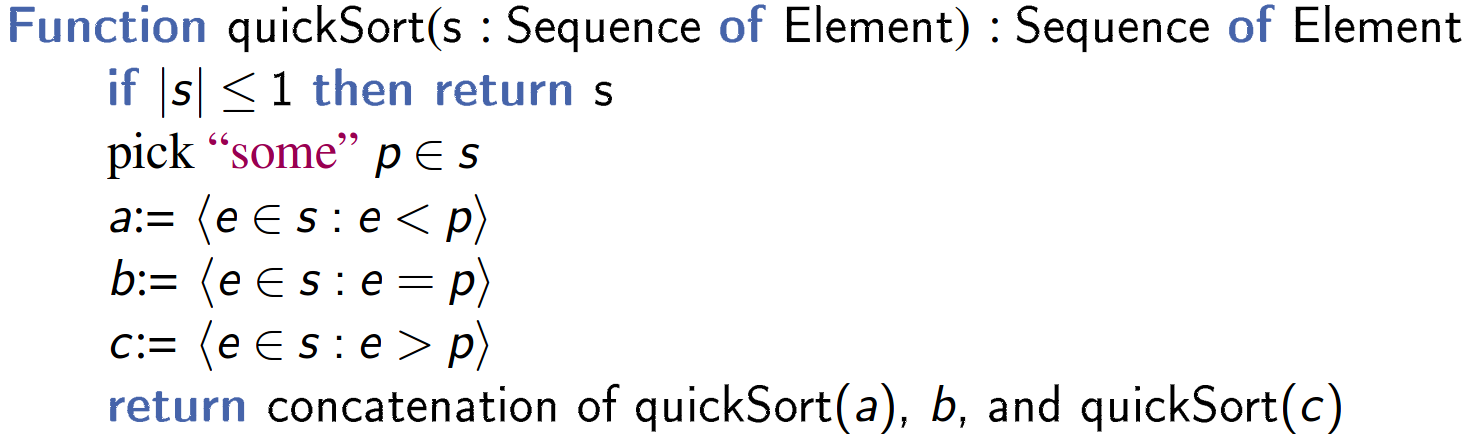
\includegraphics[width=\textwidth]{qsort_theory}

\only<1>{Beispiel: 5, 1, 0, 2, 4, 3, 6

Pivotwahl: Rechts}

\only<2>{Was ist eine Worst-Case-Eingabe, wenn als Pivot immer das rechte Element gewählt wird?}

\only<3>{Was ist eine Best-Case-Eingabe mit sieben Elementen, wenn als Pivot immer das rechte Element gewählt wird?}

\only<4>{Wie muss man das Pivot wählen, um eine aufsteigend sortierte Folge schnell zu sortieren?}

\only<5>{Wie wählt man das perfekte Pivot?

Ist das praktikabel?}

\only<6>{Welche Pivotwahl-Heuristik würdet ihr wählen, wenn ihr Quicksort implementieren müsstet?}
\end{frame}

\begin{frame}{Exkurs: \texttt{std::sort}}
\begin{itemize}
\item<1-> Standardfunktion aus der C++-STL
\item<1-> Der vermutlich meistbenutzte Sortieralgorithmus der Welt
\vspace{1em}
\item<2-> Funktionsweise:
\begin{itemize}
\item Startet mit halbrekursivem median of three Quicksort
\item Wenn der Quicksort eine Partitionsgröße kleiner oder gleich 16 erreicht, wird auf Insertionsort gewechselt
\item Wenn die Rekursionstiefe vom Quicksort $2 \log_2(n)$ übersteigt, wird für die entsprechende Partition auf Heapsort gewechselt
\item Der Heapsort wird ausgeführt, bis der Heap die Größe 16 hat, dann wird auf Insertionsort gewechselt
\end{itemize}
\end{itemize}

\pause
\pause

\only<1-3>{Warum startet man mit Quicksort?}

\only<4>{Warum benutzt man auf kleinen Partitionen Insertionsort?}

\only<5>{Warum benutzt man Heapsort?}
\end{frame}

\begin{frame}{Quicksort (konkret)}
\begin{columns}
\begin{column}{0.65\textwidth}
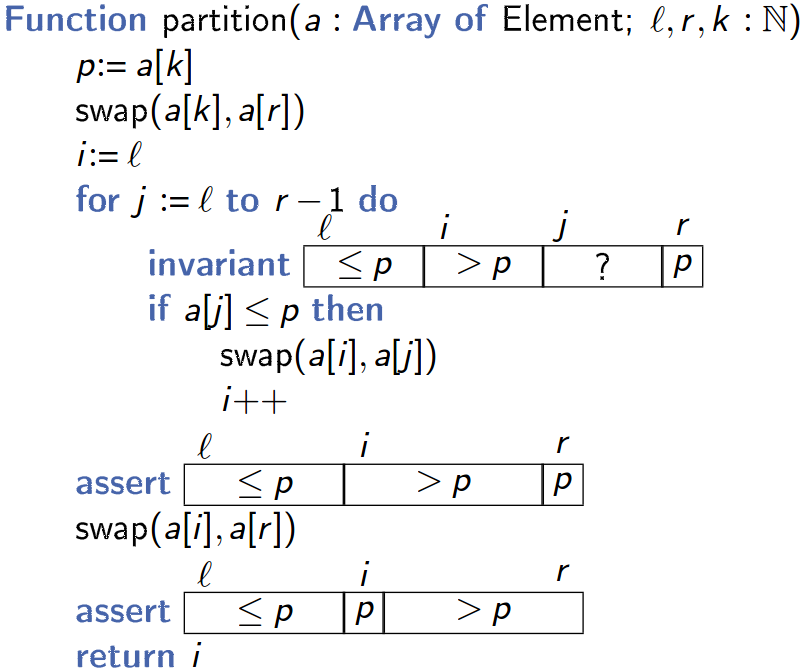
\includegraphics[width=\linewidth]{qsort_partition}
\end{column}
\begin{column}{0.35\textwidth}
\only<1>{Beispiel:\linebreak 3, 1, 5, 6, 4, 1, 3

\vspace{1em}
Pivotwahl: Rechts}

\only<2>{Was passiert, wenn alle Elemente gleich sind?}

\only<3>{Was kann man machen, um diesen Worst-Case zu verhindern?}
\end{column}
\end{columns}
\end{frame}

\begin{frame}{Bucketsort}
\begin{columns}
\begin{column}{0.5\textwidth}
1. Elemente ihren Buckets zuordnen:

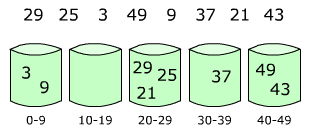
\includegraphics[width=\linewidth]{Bucket_sort_1}

\vspace{1em}
2. Innerhalb der Buckets sortieren:

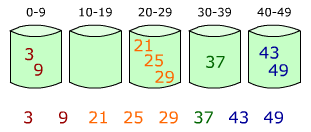
\includegraphics[width=\linewidth]{Bucket_sort_2}
\end{column}
\begin{column}{0.5\textwidth}
\only<1>{Wie sortiert man innerhalb der Buckets?}

\only<2>{Angenommen, es gibt eine Funktion $f$, die jedem Element in $O(1)$ Zeit sein Bucket zuordnet. Wie ist die Best-Case-Laufzeit von Bucketsort?}

\only<3>{Angenommen, es gibt eine Funktion $f$, die jedem Element in $O(1)$ Zeit sein Bucket zuordnet. Wie ist die Worst-Case-Laufzeit von Bucketsort?}

\only<4>{Angenommen, es gibt eine Funktion $f$, die jedem Element in $O(1)$ Zeit sein Bucket zuordnet. Wie ist die Average-Case-Laufzeit von Bucketsort?}
\end{column}
\end{columns}
\end{frame}

\begin{frame}{Ende}

\end{frame}


\end{document}
